\chapter{Empirical Analysis of Complexity}

\label{chap:analysis}

\section{Generation of Problem Instances}

There has been extensive research on synthesis of knapsack problem instances. Pisinger \cite{Pisinger:2005:HKP:1063636.1063640} explored knapsack problem instances on several popular algorithms and showed that problem instances with strongly-correlated weights and profits are hardest problems to solve. To properly analyze SKPDP it's important to make sure that the knapsack problem instances that we use are not contrived and covers the input domain. We also have to generate the problem instances systematically when we are trying to analyze the impact of a particular attribute (i.e. correlation between weight and profit values) of problem instances on SKPDP. The attributes of the problem instances that we mainly focus on are, 

\begin{itemize}
\item The portion of the items that fit into the capacity
\item The distribution of the weights
\item The correlation between the weights and profits
\end{itemize}

We discuss this attributes in more details below.
\subsection{The portion of the items that fit into the capacity}
Before generating the problem instances for range of $N$ and $C$ values, we must decide how many items out $N$ should fit into the capacity $C$. If we decide that half of the items ($N/2$) should fit into the capacity then the average weight of all the items should be,
\[
W_{avg} = \frac{2C}{N}
\]

\subsection{The distribution of the weights}
Once we have the average weight ($W_{avg}$) we need to take a distribution of the weights. We used two different types of distribution. First, we used normal distribution with a mean of $W_{avg}$ and standard deviation of $0.3$. We also used a log-normal distribution with a mean of $W_{avg}$ while making sure that the largest weight ($W_{max}$) is close to $C$. This is to analyze the impact of very large weights on SKPDP.

\subsection{The correlation between the weights and profits}
When the ratio of weights and profits of all the items of knapsack problem is a constant we end up with the hardest problem instance. It essentially becomes a subset-sum problem. We want to see the impact of correlation between weights and profits on SKPDP. So, we generated problem instances with different levels of correlation between weights and profits. For that purpose we set the profits to be a constant factor larger than the weights and introduce a small noise value. The noise is used to adjust the correlation between the weights and profits.
\[
profit = alpha * weight + \text{ random integer in the range } [-noise*W_{avg},noise*W_{avg}]
\]









\section{Potential Gain}
We explore the computational gain of the SKPDP over the conventional 0/1-KPDP.
For SKPDP to be useful, the number of operations done by the sparse algorithm
must be significantly less that the dense version.  The number of iterations
needed to generate one row of the sparse table is equal or less than twice the
size (number of pairs) of the previous row.  So, the total number of
operations needed to generate the whole sparse table is a constant factor of
the total number of pairs/critical points in the generated sparse table.  The
more sparse the sparse table is for a certain problem instance the more
performance gain we can expect.  We define potential performance gain as,

\begin{align}
  \label{eq:2}
  \text{gain} &= 1 - \frac{\text{no.\ of iterations needed for
                SKPDP}}{\text{no.\ of iterations needed for 0/1-KPDP}}
                \nonumber \\
              &\approx 1 - \frac{\text{no. of iterations needed for
                SKPDP}}{2NC} \\
  [\text{because}&\text{, we are using memory efficient version of KPDP}]
                   \nonumber
\end{align}

Notice that according to (\ref{eq:2}), maximum performance gain we can
theoretically achieve is 1, positive values of gain implies that SKPDP should
perform better than conventional 0/1-KPDP and negative values of gain implies
that SKPDP should perform worse that conventional 0/1-KPDP.

In figure \ref{fig:gain1} we plot potential gain against problem instances
with capacity ranging from $2^{12}$ to $2^{30}$ and number of items ranging
from $2^7$ to $2^{12}$.  Please note that to generate the plot we used
$(18*5=)\ 90$ different 0/1-Knapsack problem instances each with items having
strongly-correlated weights and profits; a log-normal distribution of the
weight/profit values and where approximately one-eighth of the items fit into
the capacity (i.e., average weight is $8N/C$).

\begin{figure}[htbp]
\centerline{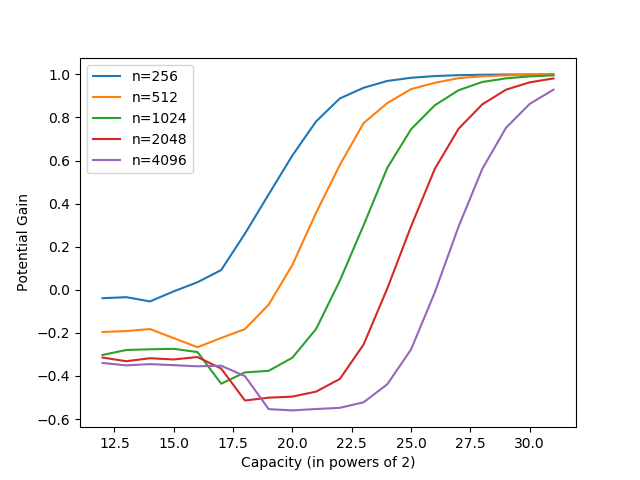
\includegraphics[width=.8\columnwidth]{images/gain1.png}}
\caption{Potential gain due to sparsity}
\label{fig:gain1}
\end{figure}

From the Figure \ref{fig:gain1} it is apparent that for large problems
instances (where capacity $C$ is much larger than $N$) we can expect
significant performance gain using SKPDP due to reduction in the number of
necessary computation to generate the sparse table.

\section{Empirical Results}
To prove our hypothesis that SKPDP performs significantly better for problem
instance where $N \ll C$ we do a log-log plot of the execution time vs the
capacity in Figure \ref{fig:time_vs_c1}.  Please note that the problem
instances in Figure \ref{fig:time_vs_c1} have the same attributes as of the
ones from the Figure \ref{fig:gain1}.  For problem instances with larger
capacity, the weight values are also proportionally larger to make sure that
the number of elements that fit into the capacity is constant for all problem
instances.  This is to make sure that our problem instances are not contrived.
 
\begin{figure}[htbp]
\centerline{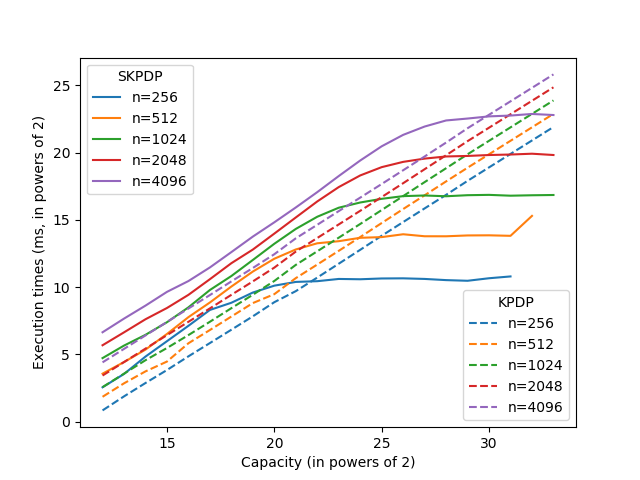
\includegraphics[width=.8\columnwidth]{images/time_vs_C1.png}}
\caption{Execution times of SKPDP for different instances of knapsack problem}
\label{fig:time_vs_c1}
\end{figure}


In the Figure \ref{fig:time_vs_c1}, the solid lines represent the execution times of SKPDP and the dashed lines represent the execution times of conventional 0/1-KPDP. We can observe that while the execution times of 0/1-KPDP stays linear with capacity $C$ (i.e. exponential with input size $log(C)$), the execution times of SKPDP becomes invariant with capacity. So, for problem instances where $N \ll C$, we can achieve exponential performance gain using SKPDP over 0/1-KPDP. SKPDP is a constant factor worse compared to 0/1-KPDP where $C$ is not large enough.

In the Figure \ref{fig:twin_vs_c1}, we can observe the correlation between the iteration count and execution time of our implementation SKPDP. It is apparent from the figure \ref{fig:twin_vs_c1} that the iteration count is correlated to the execution time of SKPDP.

\begin{figure}[htbp]
\centerline{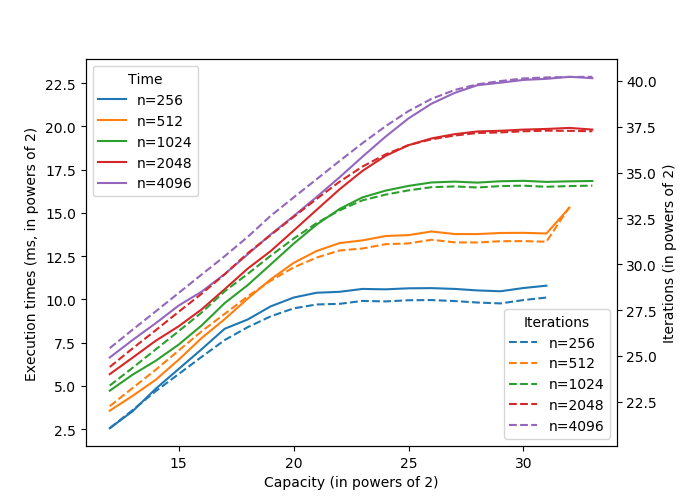
\includegraphics[width=.8\columnwidth]{images/twin_vs_C1.png}}
\caption{Comparing execution times and Op counts of SKPDP for different instances of knapsack problem}
\label{fig:twin_vs_c1}
\end{figure}

The question now is, how do we know if a problem instance has large enough value of $C$ for SKPDP to be useful over conventional KPDP? This threshold value depends on the number items ($N$), the correlation between the weights and profits and the amount elements fit into the capacity. 


\section{Impact of correlation of weights and profits}
The more strongly correlated the weights and profits of a knapsack problem instance are, the harder the problem instance is for any knapsack algorithm to solve. Figure \ref{fig:noise_vs_c1} shows that it is also true for SKPDP. When the weights and profits are perfectly correlated the SKPDP has exponential complexity. As we increase the noise value, thus reducing the correlation between weights and profits, we see much better performance by SKPDP. Note that the correlation of weights and profits does not impact the complexity of conventional 0/1-KPDP. On the other hand, even with fairly strong correlation between weights and profits we can see exponential performance improvement by SKPDP.

\begin{figure}[htbp]
\centerline{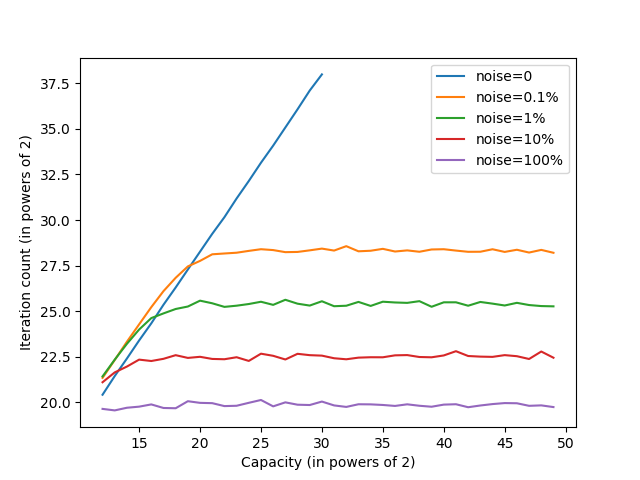
\includegraphics[width=.8\columnwidth]{images/noise_vs_C1.png}}
\caption{Iteration count of SKPDP for different levels of correlation between the weights and profits; For all problem instances $N = 256$ and $W_{avg} = \frac{8C}{N}$}
\label{fig:noise_vs_c1}
\end{figure}
\newpage



\section{Impact of the portion of items that fit into the capacity}
Figure \ref{fig:fits_vs_c1} compares the iteration counts of knapsack problem instances with 4 different average weights of the items. When we want half of the items to fit into the capacity (on average), we make sure that $W_{avg}=\frac{2C}{N}$; when we want 1/4-th of items to fit into the capacity, we make sure that $W_{avg}=\frac{4C}{N}$ and so on. From the figure \ref{fig:fits_vs_c1} it is apparent that for any given $N$ and $C$ values, problem instances with higher values of $W_{avg}$ have more sparsity. Again, note that this attribute does not impact the complexity of conventional 0/1-KPDP.


\begin{figure}[htbp]
\centerline{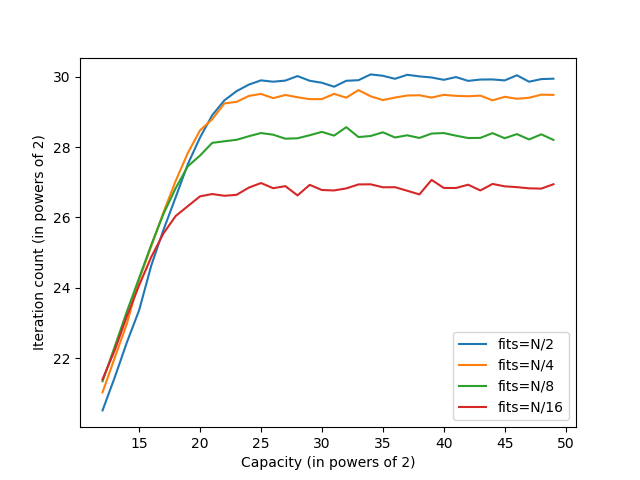
\includegraphics[width=.8\columnwidth]{images/fits_vs_C1.png}}
\caption{Iteration count of SKPDP for different portions of the items fitting into the capacity; For all problem instances $N = 256$ and $noise = 0.1\%$}
\label{fig:fits_vs_c1}
\end{figure}

